%% The first command in your LaTeX source must be the \documentclass command.
%%
%% Options:
%% twocolumn : Two column layout.
%% hf: enable header and footer.
\documentclass[
% twocolumn,
% hf,
]{ceurart}

%%
%% One can fix some overfulls
\sloppy

%%
%% Minted listings support 
%% Need pygment <http://pygments.org/> <http://pypi.python.org/pypi/Pygments>
\usepackage{listings}
\usepackage{biblatex}
\addbibresource{sample-ceur.bib}
%% auto break lines
\lstset{breaklines=true}

\usepackage[acronym]{glossaries}

\newacronym{auc}{AUC}{Area under the receiver operating characteristic curve}
\newacronym{wkt}{WKT}{Well Known Text}
\newacronym{noaa}{NOAA}{National Oceanic and Atmospheric Administration}
\newacronym{nlcd}{NLCD}{National Land Cover Database}
\newacronym{idw}{IDW}{Inverse Distance Weighting}
\newacronym{scec}{SCEC}{State Climate Extremes Committee}
\newacronym{ok}{OK}{Ordinary Kriging}
\newacronym{uk}{UK}{Universal Kriging}
\newacronym{loocv}{LOOCV}{Leave-One-Out-Cross-Validation}
\newacronym{rmse}{RMSE}{Root Mean Squared Error}
\newacronym{osm}{OSM}{OpenStreetMap}
\newacronym{de-9im}{DE--9IM}{Dimensionally Extended 9-Intersection Model}
\newacronym{crs}{CRS}{Coordinate Reference System}
\newacronym{id}{ID}{Identifier}
\newacronym{wgs84}{WGS84}{World Geodetic System 1984}
\newacronym{api}{API}{Application Programming Interface}
\newacronym{xgb}{XGB}{XGBoost}
\newacronym{csv}{CSV}{Comma-seperated values}
\newacronym{ml}{ML}{Machine Learning}
\newacronym{kg}{KG}{Knowledge Graph}
\newacronym{stkg}{STKG}{Spatio-Temporal Knowledge Graph}

%%
%% end of the preamble, start of the body of the document source.
\begin{document}

%% The first command in your LaTeX source must be the \documentclass command.
%%
%% Options:
%% twocolumn : Two column layout.
%% hf: enable header and footer.
\documentclass[
% twocolumn,
% hf,
]{ceurart}

%%
%% One can fix some overfulls
\sloppy

%%
%% Minted listings support 
%% Need pygment <http://pygments.org/> <http://pypi.python.org/pypi/Pygments>
\usepackage{listings}
\usepackage{biblatex}
\addbibresource{sample-ceur.bib}
%% auto break lines
\lstset{breaklines=true}

\usepackage[acronym]{glossaries}

\newacronym{auc}{AUC}{Area under the receiver operating characteristic curve}
\newacronym{wkt}{WKT}{Well Known Text}
\newacronym{noaa}{NOAA}{National Oceanic and Atmospheric Administration}
\newacronym{nlcd}{NLCD}{National Land Cover Database}
\newacronym{idw}{IDW}{Inverse Distance Weighting}
\newacronym{scec}{SCEC}{State Climate Extremes Committee}
\newacronym{ok}{OK}{Ordinary Kriging}
\newacronym{uk}{UK}{Universal Kriging}
\newacronym{loocv}{LOOCV}{Leave-One-Out-Cross-Validation}
\newacronym{rmse}{RMSE}{Root Mean Squared Error}
\newacronym{osm}{OSM}{OpenStreetMap}
\newacronym{de-9im}{DE--9IM}{Dimensionally Extended 9-Intersection Model}
\newacronym{crs}{CRS}{Coordinate Reference System}
\newacronym{id}{ID}{Identifier}
\newacronym{wgs84}{WGS84}{World Geodetic System 1984}
\newacronym{api}{API}{Application Programming Interface}
\newacronym{xgb}{XGB}{XGBoost}
\newacronym{csv}{CSV}{Comma-seperated values}
\newacronym{ml}{ML}{Machine Learning}
\newacronym{kg}{KG}{Knowledge Graph}
\newacronym{stkg}{STKG}{Spatio-Temporal Knowledge Graph}

%%
%% end of the preamble, start of the body of the document source.
\begin{document}

%%
%% Rights management information.
%% CC-BY is default license.
\copyrightyear{2023}
\copyrightclause{Copyright for this paper by its authors.
  Use permitted under Creative Commons License Attribution 4.0
  International (CC BY 4.0).}

%%
%% This command is for the conference information
\conference{Second International Workshop on Linked Data-driven Resilience Research (D2R2'23) co-located with ESWC 2023, May 28th, 2023, Hersonissos, Greece}

%%
%% The "title" command
\title{Wildfire Prediction Using Spatio-Temporal Knowledge Graphs}

%%
%% The "author" command and its associated commands are used to define
%% the authors and their affiliations.
\author[1,2]{Martin B\"ockling}[%
orcid=0000-0002-1143-4686,
email=martin.boeckling@students.uni-mannheim.de,
]
\cormark[1]
\fnmark[1]
\address[1]{University of Mannheim, Data and Web Science Group,
  B6, 26, 68161 Mannheim}
\address[2]{SAP SE,
  Dietmar-Hopp-Allee 16, 69190 Walldorf}

\author[1]{Heiko Paulheim}[%
orcid=0000-0003-4386-8195,
email=heiko@informatik.uni-mannheim.de,
]
\cormark[1]
\fnmark[1]

\author[2]{Sarah Detzler}[%
orcid=0000-0002-7504-8856,
email=sarah.detzler@sap.com,
]
\cormark[1]
\fnmark[1]

%% Footnotes
\cortext[1]{Corresponding author.}
\fntext[1]{These authors contributed equally.}

%%
%% The abstract is a short summary of the work to be presented in the
%% article.
\begin{abstract}
  The frequency of wildfires increases yearly and poses a constant threat to the environment and human beings. Different factors, for example surrounding infrastructure to an area (e.g., campfire sites or power lines) contribute to the occurrence of wildfires. In this paper, we propose using a \gls*{stkg} based on \gls*{osm} data for modeling such infrastructure. Based on that knowledge graph, we use the RDF2vec approach to create embeddings for predicting wildfires, and we align different vector spaces generated at each temporal step by partial rotation. In an experimental study, we determine the effect of the surrounding infrastructure by comparing different data composition strategies, which involve a prediction based on tabular data, a combination of tabular data and embeddings, and solely embeddings. We show that the incorporation of the \gls*{stkg} increases the prediction quality of wildfires.
\end{abstract}

%%
%% Keywords. The author(s) should pick words that accurately describe
%% the work being presented. Separate the keywords with commas.
\begin{keywords}
  Knowledge Graph Embeddings \sep
  Spatio-Temporal Knowledge Graph \sep
  RDF2vec \sep
  Wildfire Prediction
\end{keywords}

%%
%% This command processes the author and affiliation and title
%% information and builds the first part of the formatted document.
\maketitle

\section{Introduction}
Wildfires as a natural phenomenon have increased in their frequency as well as in their damage to the territory of the United States. Wildfires are unplanned fires which can have natural causes, human-related causes as also have their origin in planned fires. When analyzing the period from 1960 to 2021, the top five highest burned areas by wildfires per year were all after 2006. For the year 2021 in total, 58,968 wildfires have been detected over the complete territory of the United States with a burned area around 7,100,000 acres \cite{Hoover.2021}. The prediction of wildfires relies on factors which can be characterized as complex systems, in which different influence factors and surrounding factors are present in contributing to the occurrence of wildfires \cite{Pastor.2003}. A base argumentation for complex systems in geography was determined by Tobler's first law, for which he stated that “Everything is related to everything else, but near things are more related than distant things” \cite{Tobler.1970}. Our approach, which builds the base for the wildfire prediction in this paper, builds up on this premise and follows the hypothesis that an involvement of a \gls*{kg} is beneficial to predicting wildfires. Wildfire prediction in the context of this paper represents the prediction of a wildfire occurrence for the given input types of one given spatial grid cell to the specified time step.

\section{Related Work} \label{sec:RelatedWork}
For the topic of wildfire prediction, a variety of different research papers exist. \textcite{Nami.2018} calculate the probability of wildfires for the Hyrcanian ecological region. For the probability prediction of wildfires temperature variables, landscape information and spatial property data are incorporated into the final dataset. All variables are modeled on a regular spatial grid to integrate them into a unified dataset. The spatial property data is organized by using distance bins, unfolding into a category for each bin \cite{Nami.2018}. A different study of wildfire prediction is conducted for the territory of South Korea. It includes landscape data, weather data as also social-economic data and the distance to spatial property data. Each dataset is transformed together by using a regular spatial grid. The modeling is performed by using a Maximum Entropy and Random Forest classifier \cite{Kim.2019}.

Different research papers have used \gls*{osm} data to construct a Spatial Knowledge Graph or enrich other Knowledge Graphs with data from \gls*{osm}. \textcite{Dsouza.2021} have constructed a Knowledge Graph called WorldKG, globally integrating the \gls*{osm} data into a Knowledge Graph. For the construction of WorldKG, the data is derived from \gls*{osm} and inserted into a hierarchical structure using the key-value pairs from \gls*{osm}. The Ontology of WorldKG uses the keys as classes and the key-value pairs as subclasses. Furthermore, the spatial object structures are captured regarding the spatial geometry types and the exact structure of the geometry types stored in the \gls*{wkt} format. In total, the published Knowledge Graph consists of 828,550,751 triples and 113,444,975 total entities \cite{Demartini.2021}. \textcite{Johnson.2022} have created a concept for different Knowledge Graphs consisting of \gls*{osm} data, social-economic data and flood data. For the different datasets modeled, the structure of the Knowledge Graph varies in the structure. For the social-economic dataset the data is divided into fixed regions, for the \gls*{osm} data the overall geometry structure of single buildings \cite{Johnson.2022}. The paper of \textcite{Wu.2022} uses \gls*{noaa} weathers data to model it into a knowledge graph. For each weather station, the data type together with the location is modeled into a Knowledge Graph. Furthermore, the position of each weather station is encoded into two separate entities separated between longitudes and latitudes. Furthermore, the Knowledge Graph is enriched together with the data derived from \gls*{osm} and Wikidata \cite{Wu.2022}.

Given the presented papers that were available for our research, the methodology used in this paper is the first to create a \gls*{stkg} with \gls*{osm} data modeled on a spatial grid over continuous time steps. Especially, other papers and approaches do not model their \gls*{kg} using a spatial grid to capture dynamic changes over continuous time steps. The use of \glspl*{kg} for wildfire prediction is, to the best of our knowledge, the first time used to model spatial relationships between geographic entities. %In section \ref{cha:Approach} we outline our approach used for this paper.

\section{Approach} \label{cha:Approach}
For this paper, the approach for our research results in three different research datasets that we use for predicting wildfires. The first dataset, named BaseCase dataset, includes tabular data from a variety of different data sources, which we integrate by using a spatial grid. This approach is consistent with the current state of the art and is used similarly by the presented work in section \ref{sec:RelatedWork} \cite{Nami.2018, Kim.2019}. A general overview of our approach can be found in figure \ref{fig:Approach}. The second dataset, which is named HybridCase dataset, uses as a base for the dataset structure the BaseCase dataset. In addition, the embeddings derived from the \gls*{stkg} using RDF2vec are introduced to the dataset as new columns. The third dataset is using solely the embeddings derived from the constructed \glspl*{stkg} by integrating every dataset into the \gls*{kg}. In the following paragraphs, the procedure for our paper is outlined in detail based on figure~\ref{fig:Approach}.

\begin{figure}[t]
	\centering
	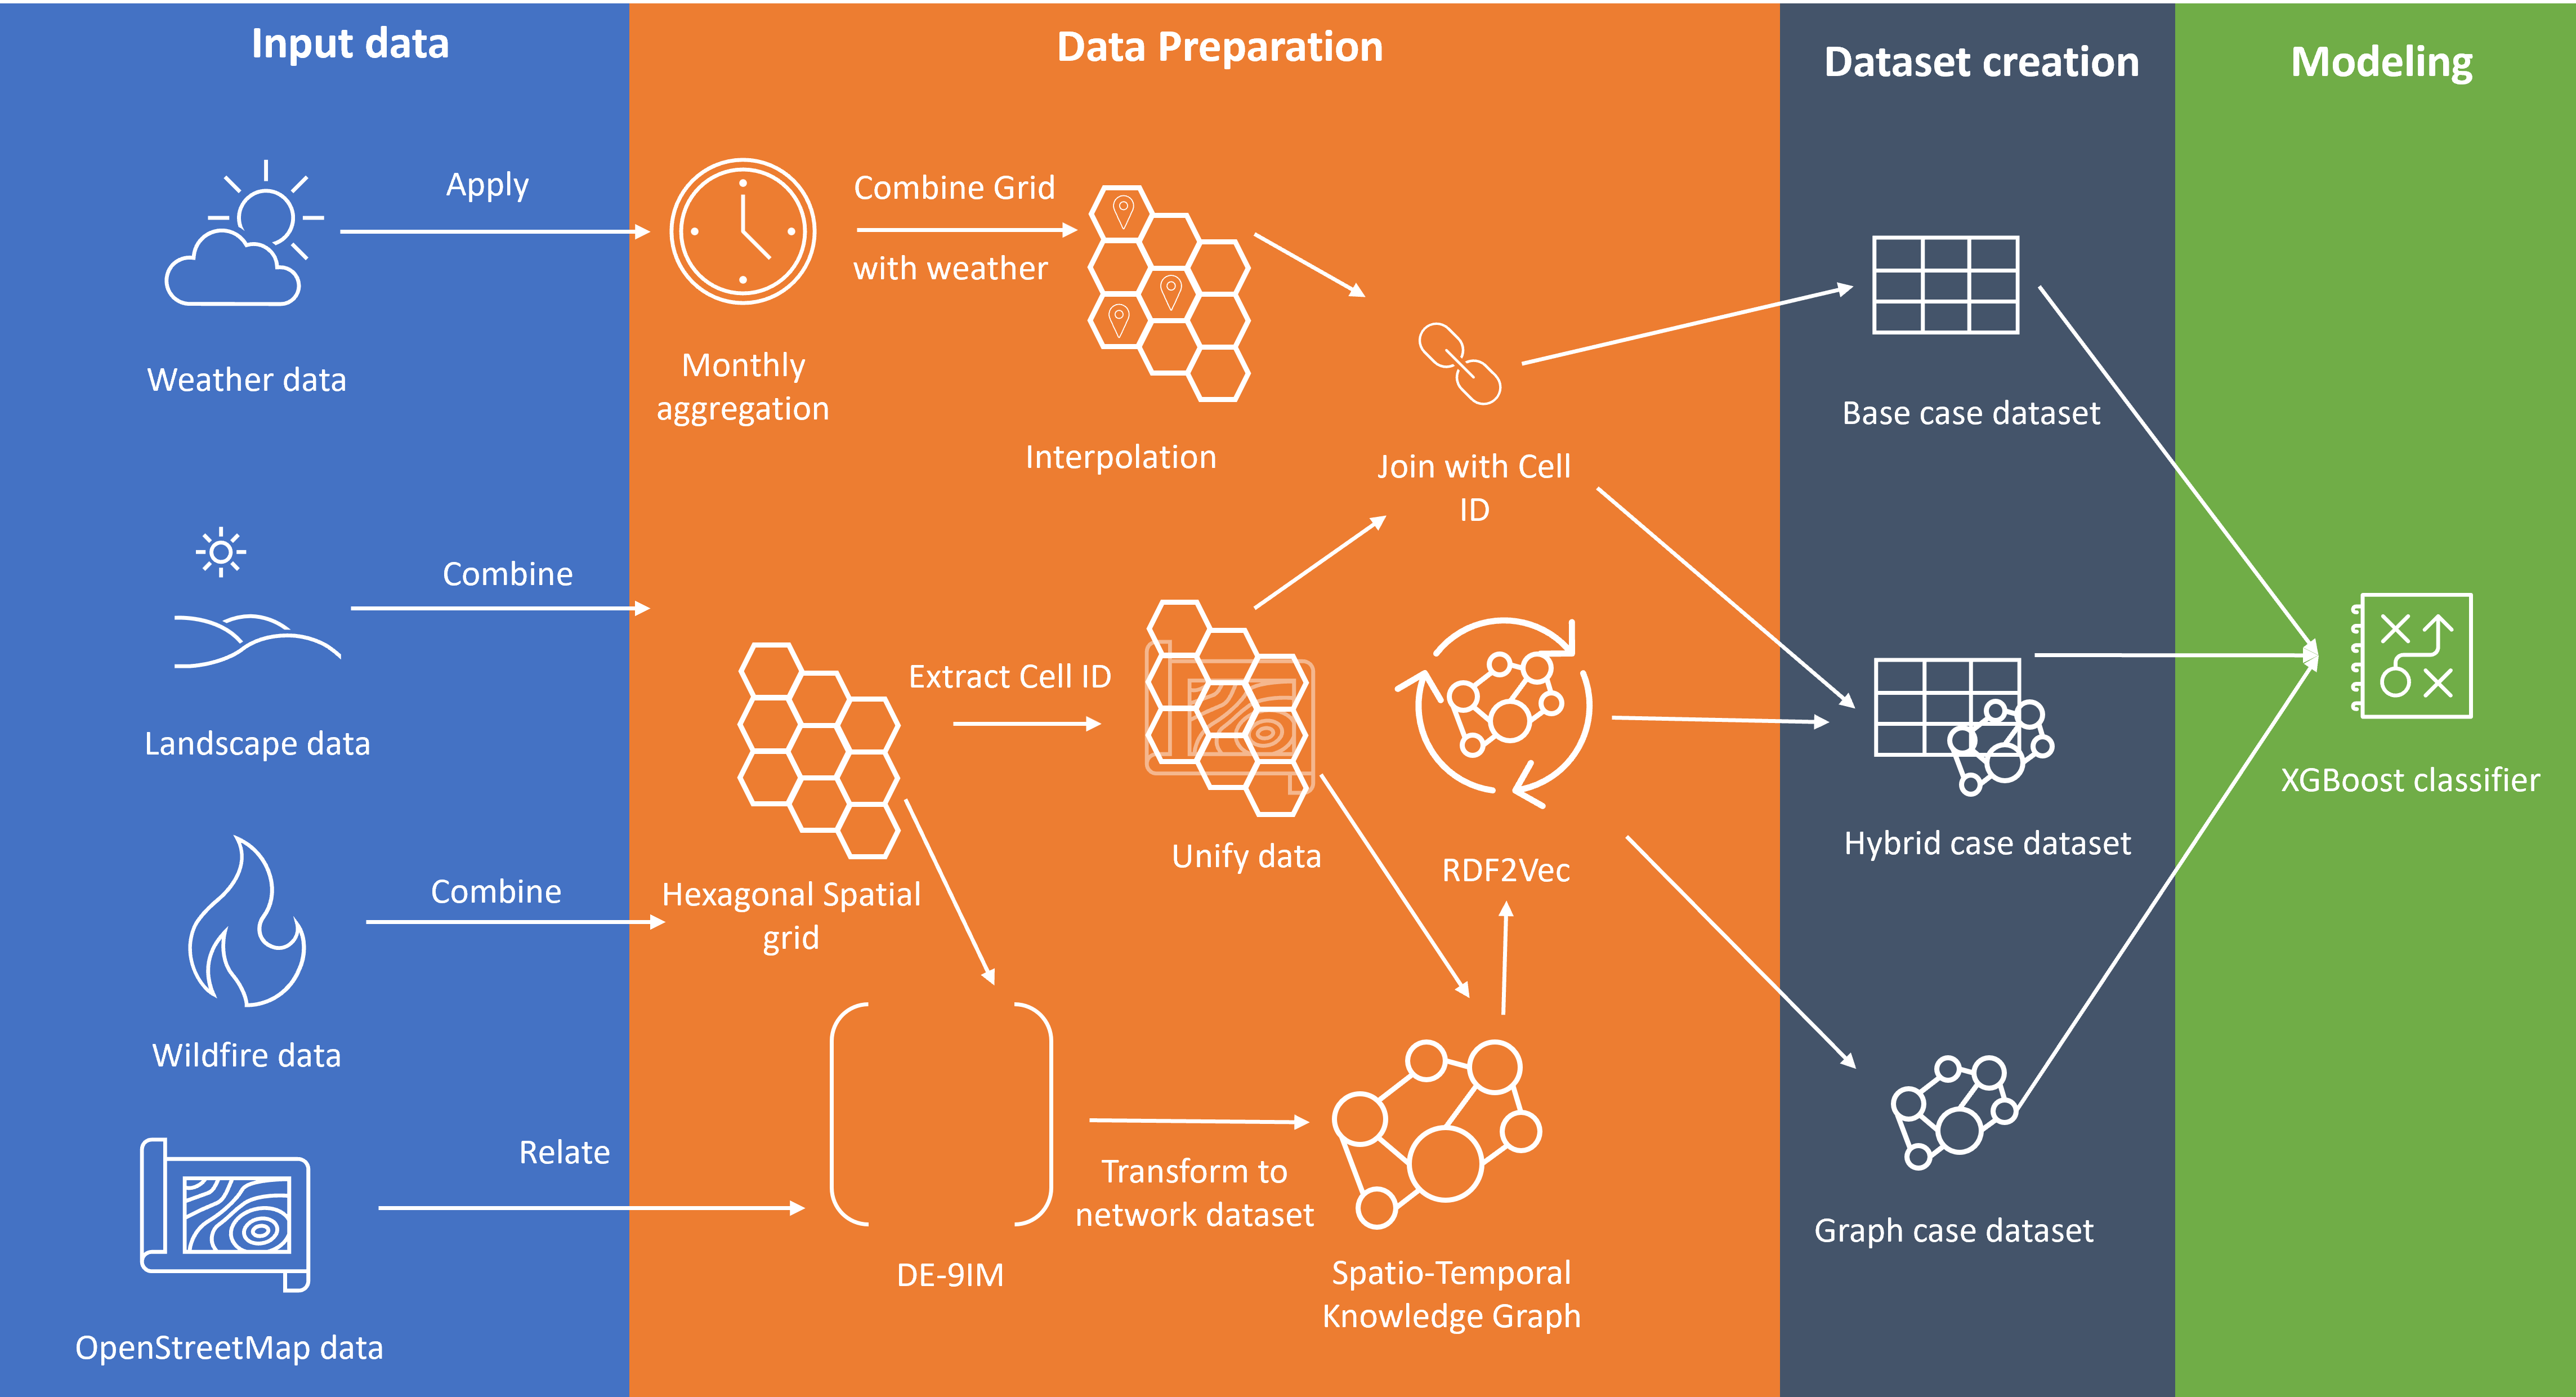
\includegraphics[width = 0.85\textwidth]{img/Approach.png}
	\caption{Approach for the wildfire detection performed in this paper}
	\label{fig:Approach}
\end{figure}

Besides the wildfire data \cite{Giglio.2015} which is used to mark a wildfire occurrence, weather data \cite{Menne.2012}, landscape data \cite{Yang.2018} as also a selection of \gls*{osm} data \cite{OpenStreetMapcontributors.2017}\footnote{Details of \gls*{osm} data selection can be found under the following page \url{https://github.com/MartinBoeckling/WildfirePredictionSTKG/blob/main/wildfirearea/OSMTags.md}.} is used for the wildfire prediction datasets. The wildfire prediction in this paper is based on monthly data. If not all datasets cover the monthly periods, we either aggregate the data to a monthly basis or expand the data to a monthly basis if it does not cover all months in the period of 2010-2021. For the expansion of the datasets, we duplicate the data associated to a specific year onto the monthly basis. The extraction of the specified data can be found on the first layer in figure \ref{fig:Approach}.

As we want to integrate data sources of different structure, we use spatial grids to unify the data and divide the research region into different singular cells \cite{Rigaux.2001}. For the created spatial grid, we use a regular geometric structure for our grid, as those are best suited for the data types we are using \cite{Rigaux.2001}. For the selection of the geometric base structure, we use hexagons, as those allow us to aggregate data more accurately \cite{Wang.2018} and provide an equal distance to each of its neighbors \cite{Birch.2007}. By tessellating the territory of California, we construct a hexagonal spatial grid which is spanned over the complete territory of California. Each of the individual grid cells within the spatial grid is assigned with an unique \gls*{id}.

For the individual datasets, a different data preparation is needed to align the datasets for a monthly wildfire prediction. The weather dataset captures the daily weather for the period of 2010 to 2021. Therefore, the weather data needs to be aggregated on a monthly basis so that the period is matching to the required period. The selection of the aggregation method is derived by the meaning of the individual variables. If the average temperature is captured in a variable, a mean aggregation is applied to the individual station for the complete month. This paradigm is used across all variables for the weather dataset. After the aggregation of the weather data on a monthly basis, we interpolate the weather to expand the point-wise measurement over the territory of California. For the interpolation of the weather data, we rely on a combination of \gls*{idw} and Kriging. The Kriging interpolation showcased to have an accurate data representation for the interpolation \cite{Pede.2018}. However, Kriging produces also values which are above the global extreme values \cite{Matheron.1963}. For our paper, the assumption is made that the simple limitation would perform worse than the \gls{idw} performed interpolation. Therefore, the replacement of invalid values violating the global limit is performed by an \gls{idw} interpolation.

For the landscape data, the dataset has data for the years 2011, 2013, 2016 and 2019. As the landscape data is on a more fine granular level, we aggregate the values of the landscape data to our created grid using the majority vote aggregation, for which the landscape category with the highest fraction in the grid cell is assigned to the respective grid cell. Afterward, the data is expanded on a monthly basis to capture each individual year for the covered period.

For the creation of our \gls*{stkg}, we incorporate three different data preparations depending on the structure of the incorporated datasets. The base for our \gls*{stkg} is the neighbor relation between each spatial grid cell. For each of the individual grid cells, the neighboring relation is modeled. Between the \gls*{osm} dataset with its geometries and the individual grid cells, the relationship is determined by using the \gls*{de-9im} method \cite{Clementini.1993}. From the methodology, in total seven different relations are derived: Contains, covered by, covers, crosses, intersects, overlaps and touches. An explanatory situation for the modeled relation is displayed in figure \ref{fig:RelationKG}.

\begin{figure}[t]
	\centering
	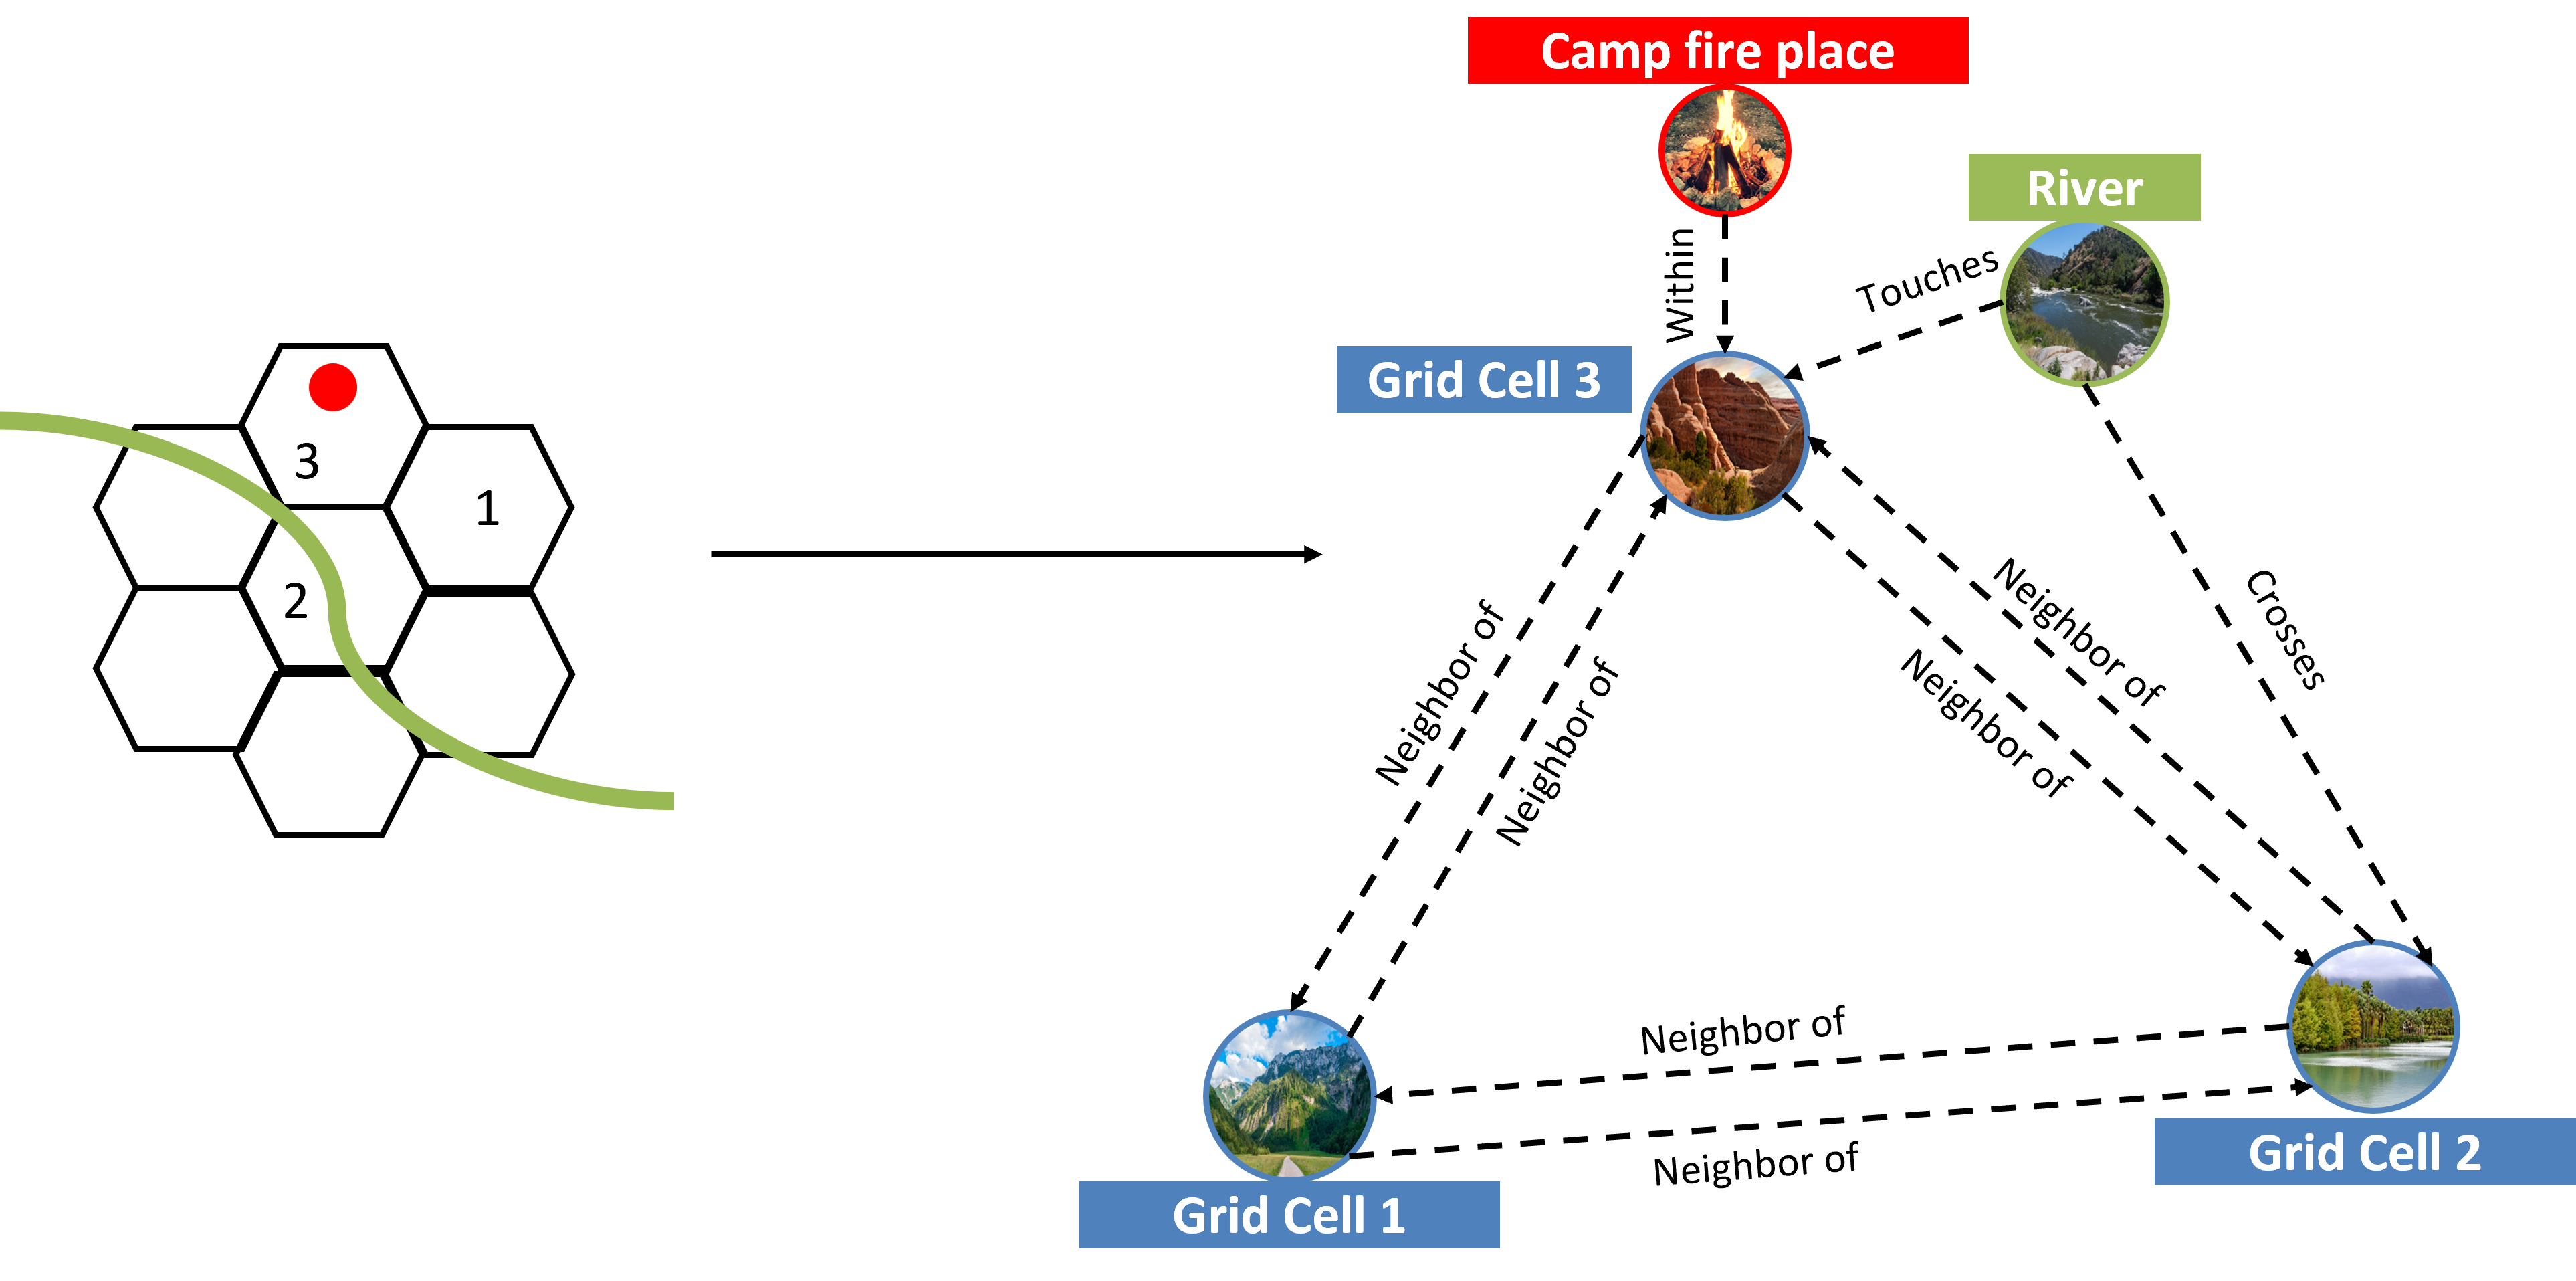
\includegraphics[width = 0.8\textwidth]{img/RelationGrid.png}
	\caption{\gls*{kg} relation modeled from datasets}
	\label{fig:RelationKG}
\end{figure}

For values within the tabular dataset including all used variables, the values are transposed into individual vertices, in which the respective object \gls*{id} is the subject, the variable of the value builds the predicate and the value itself is the object. Those individual transformations are aligned on the monthly basis, so that the \gls*{stkg} cover the necessary monthly period for the years 2010 to 2021. The outlined approach enables the possibility to model relationships not only locally, but also between neighbors. This provides the possibility to realize the first law of geography.

To make the constructed \gls*{stkg} applicable for the wildfire prediction, we transform the data into a vector representation. For the vector generation, we use the RDF2vec method \cite{Ristoski.2016}. The created \glspl*{stkg} differ for the HybridCase and NetworkCase dataset. For the HybridCase dataset, only the prepared \gls*{osm} data is used, for the NetworkCase dataset the \gls*{stkg} with each dataset except the wildfire dataset is used for the vector generation. The RDF2vec has two important parameters, i.e., the maximum walk length and the maximum number of walks per entity. For the walk length, the maximum steps necessary to reach all entities related to the neighboring grid cell from one spatial grid cell is a walk distance of four. Due to the limit in available memory storage, the maximum number of walks extracted per entity is set to 1,024. As we use the RDF2vec approach for each temporal interval, we need to align the produced embeddings to a common projection. For the alignment of the embeddings, we use a methodology relying on the orthogonal Procrustes problem, where a mapping between two matrices is estimated and then applied to the matrix, which needs to be aligned \cite{Hamilton.2016}.

Each individual dataset is joined using the grid cell \gls*{id} and the month. As discussed earlier in this paragraph, we differentiate between three different dataset constellations. For the BaseCase dataset, this data consists of the prepared tabular datasets from the landscape data, weather data and wildfire data. The HybridCase dataset uses the BaseCase dataset as a base and expands the dataset with the generated embeddings for the \gls*{osm} based \gls*{stkg}. The NetworkCase dataset uses the embeddings derived from the combined \gls*{stkg} consisting of landscape data, weather data and \gls*{osm} data.

After the creation of the datasets, we classify wildfire events using the \gls*{xgb} algorithm \cite{Chen.2016}. As \gls*{xgb} comes with a variety of different parameters, we use a Bayesian Optimization technique to tune a selection of \gls*{xgb} hyperparameters using the BayesianOptimization python package \cite{Nogueira.2014}. Bayesian Optimization for hyperparameter tuning showed promising results in comparison to other Hyperparameter Tuning methods regarding the speed of finding the optimal solution \cite{Snoek.2012}. For our hyperparameter tuning, we perform ten random iterations and afterward perform 50 iterations using the Bayesian Optimization. %In picture \ref{fig:Approach} we outline our general approach used in this paper.

\section{Evaluation}
To evaluate the performance for all different datasets, we determine the effect of the classification model by comparing the performance with the F1 score, as it provides a better representation than the accuracy \cite{Maimon.2010}. In subsection \ref{cha:EvaluationProtocol} we determine the exact testing procedure for all dataset constellations.

\subsection{Evaluation Protocol}\label{cha:EvaluationProtocol}
For the evaluation of the different datasets, we define the train split for all data values from 2010 to 2019. The test dataset contains all rows related to the years 2020 and 2021. As the occurrences of wildfires are with only 0.58\% present in the train dataset, we consider a Random Oversampling to rebalance the train dataset. As we tune our hyperparameters, we perform a cross validation of the data. Due to the time dependency in the data, we cannot directly use a cross validation function, as we could base our prediction on future values for the past. Therefore, we split the dataset based on the time for our cross validation. For each training iteration, we only rebalance the dataset that is used for training, whereas the datasets for validation and test are not rebalanced. 

For the hyperparameter tuning, we use a subset of the available parameters within \gls*{xgb}. The selection of the hyperparameter variables with its ranges is based on the recommendation from the official \gls*{xgb} website\footnote{Under the \href{https://xgboost.readthedocs.io/en/stable/tutorials/param_tuning.html}{\gls*{xgb} website}, the recommended variables are outlined}. The \gls*{xgb} classifier uses a fixed seed to make the results reproducible. As an objective for the algorithm, we use the binary:logistic configuration together with the parameter tree\_method and value hist. For the overall validation routine, we use the F1 score to determine the best parameter combination, to determine the optimal parameters for the different dataset combinations \footnote{The search space for the parameter optimization includes the parameters min\_child\_weight: [0, 100], max\_depth: [0, 50], subsample: [0.01, 1], colsample\_bytree: [0.01, 1.0], gamma: [0, 50], n\_estimators: [50, 1000]}. 


% In table \ref{tab:parameterSetting} the overview of the tuned parameters with the value range can be found.

% \begin{table*}[h]
% 	\caption{Hyperparameter selection together with parameter range}
% 	\label{tab:parameterSetting}
% 	\begin{tabular}{p{0.65\textwidth}p{0.3\textwidth}}
% 		\toprule
% 		Parameter & Parameter range\\
% 		\midrule
% 		min\_child\_weight &  [0, 100]\\
% 		max\_depth & [0, 50] \\
% 		subsample & [0.01, 1] \\
% 		colsample\_bytree & [0.01, 1.0] \\
%         gamma & [0, 50] \\
%         n\_estimators & [50, 1000] \\
% 		\bottomrule
% 	\end{tabular}
% \end{table*}

\subsection{Results}\label{cha:Results}
For the comparison between the different dataset constellations, we compare in total four different datasets. The dataset BaseCase does involve the tabular data as described in subsection \ref{cha:Approach}. For the hybrid data constellation, we combine the embeddings together with the tabular data represented in the HybridCase dataset. The third data constellation is based solely on the generated embeddings derived from the constructed \gls*{stkg} using all datasets. In table \ref{tab:resultModeling} the results of the wildfire prediction after the hyperparameter tuning are outlined.
\begin{table*}[t]
	\caption{Model results after hyperparameter tuning, the highest F1 score is marked bold}
	\label{tab:resultModeling}
    \begin{tabular}{p{0.3\textwidth}p{0.09\textwidth}p{0.09\textwidth}p{0.09\textwidth}p{0.09\textwidth}p{0.14\textwidth}}
		\toprule
		Dataset \gls*{id} & True Negative & False Positive & False Negative & True \linebreak Positive & F1 Score\\
		\midrule
		BaseCase & 718,695 & 82,178 & 13,538 & 25,523 & 0.3478$\pm$0.0010 \\
		HybridCase & 729,614 & 71,259 & 13,160 & 25,901 & \textbf{0.3803}$\pm$0.0011 \\
		NetworkCase & 797,829 & 3,068 & 38,834 & 227 & 0.0107$\pm$0.0002 \\
		\bottomrule
	\end{tabular}
\end{table*}

%To put the results into context, we reflect our results critically in section \ref{cha:Discussion}. For the wildfire predictions, we discuss the limitations of our research together with possible expansion possibilities. Furthermore, we evaluate the results based on the presented works in section \ref{sec:RelatedWork}.

\subsection{Discussion} \label{cha:Discussion}
For the selection of all datasets used in this paper, a bias regarding the \gls*{ml} results is present, as not all possible influence factors of wildfires are included. For example, long-term drought factors or social economic data, which might have a long-term effect on wildfire occurrence, are not present in the datasets \cite{Littell.2018}. Therefore, each result derived from the modeling phase needs to be critically viewed, as not all necessary influence factors for wildfires are present within the data. 

The validity of the datasets used is only partially assessed. For the weather variables, the \gls*{scec}provides extreme values for a selection of weather variables \cite{StateClimateExtremesCommittee.2022}. A filtering of anomaly-based methods is not conducted, as it could have filtered out patterns of weather extremes contributing to wildfire occurrences. 

For our \gls*{stkg} we have involved a sample of \gls*{osm} data. Compared to WorldKG created by \cite{Tempelmeier.2021} we only use a subset of data types specifically related to wildfire causes in California. This selection proposes the situation that not all possible geographic relations captured in \gls*{osm} have been determined within the territory of California. Furthermore, the \gls*{osm} data is derived on a yearly basis due to the limited performance of the \gls*{osm} \gls*{api}. As \gls*{osm} is a community-based platform similar to Wikipedia, its data is not guaranteed as complete and correct. Based on the curation process of \gls*{osm}, inconsistent data can be present as well as missing information for existing spatial properties in reality \cite{Basiri.2016}.

Our results are strictly restricted to the territory of California. In general, the constructed artifacts and performance metrics cannot be directly compared to other regions in the world, as the hexagonal grid and different other data sources are not directly transferable to other regions within the United States. An alternative solution for the spatial grid would be by using globally spanned hierarchical grids. Examples of spatial hierarchical grids are the h3 grid created by Uber and OpenEAGGR, which both would allow furthermore a consistent global integration of spatial data. Due to the limited area we investigated for this paper, both approaches have not been evaluated regarding their influence on the wildfire prediction.

Within the paper, different dataset constellations have been combined and used. For different data preparation combinations within the datasets, a change in the metrics for the prediction can be observed. However, it is important to state that due to the focus of the paper and experimental design, it is not the goal to assess which data preparation techniques help to boost the wildfire prediction generally. For the different dataset constellations, the dataset HybridCase performs significantly better than all other datasets. However, the dataset NetworkCase involving the \gls*{stkg} embeddings showcased a significant lower performance compared to the BaseCase dataset.

\section{Conclusion and Outlook}
This paper has showcased that, dependent on the data preparation, the incorporation of \gls*{stkg} embeddings has a significant effect on the prediction of wildfires. This effect has been showcased in the hybrid data constellation, where the tabular data is combined with the \gls*{stkg} embeddings. Furthermore, the performance of the data constellation where the pure Knowledge Graph embedding has been used showed a significant lower performance compared to the BaseCase data constellation. Therefore, it can be derived that the construction of the \gls*{stkg} for the network data constellation could be improved. Instead of pivoting the tabular datasets into an edge dataset, the values could be defined as node attributes, which would describe the node more accurately. Furthermore, instead of modeling a separate \gls*{stkg}, the performance could be compared to the created WorldKG created by \textcite{Tempelmeier.2021}.

For further research, additional vectorization techniques can be tested regarding the constructed knowledge graphs and compared towards the performance of a downstream task like the wildfire prediction. The different vectorization techniques could also be compared regarding their appliance to a dynamic Knowledge Graph. Examples for alternative Knowledge Graph embedding methods could be TransE, RESCAL or neural network-based embedding approaches like Semantic Matching Energy \cite{Wang.2017}. Furthermore, the Navi approach, proposed by \textcite{Krause.2022}, could be compared to the alignment used in this paper regarding its performance on wildfire detection \cite{Krause.2022}. Alternatively to the used \gls*{xgb} classifier, other classification algorithms like a Random Forest or Graph Neural Networks could be used to compare the results derived from the datasets.

%%
%% The acknowledgments section is defined using the "acknowledgments" environment
%% (and NOT an unnumbered section). This ensures the proper
%% identification of the section in the article metadata, and the
%% consistent spelling of the heading.
\begin{acknowledgments}
  Computing resources have been funded by SAP SE. Map data copyrighted OpenStreetMap contributors and available from \url{https://www.openstreetmap.org}.

\end{acknowledgments}

%%
%% Define the bibliography file to be used
\printbibliography

%%
%% If your work has an appendix, this is the place to put it.
\appendix

\section{Online Resources}

The sources for the paper are available via \\href{https://github.com/MartinBoeckling/WildfirePredictionSTKG}{GitHub}.


\end{document}

\end{document}
